%%
% Plantilla de Memoria
% Modificación de una plantilla de Latex de Nicolas Diaz para adaptarla 
% al castellano y a las necesidades de escribir informática y matemáticas.
%
% Editada por: Mario Román
%
% License:
% CC BY-NC-SA 3.0 (http://creativecommons.org/licenses/by-nc-sa/3.0/)
%%

%%%%%%%%%%%%%%%%%%%%%
% Thin Sectioned Essay
% LaTeX Template
% Version 1.0 (3/8/13)
%
% This template has been downloaded from:
% http://www.LaTeXTemplates.com
%
% Original Author:
% Nicolas Diaz (nsdiaz@uc.cl) with extensive modifications by:
% Vel (vel@latextemplates.com)
%
% License:
% CC BY-NC-SA 3.0 (http://creativecommons.org/licenses/by-nc-sa/3.0/)
%
%%%%%%%%%%%%%%%%%%%%%

%----------------------------------------------------------------------------------------
%	PAQUETES Y CONFIGURACIÓN DEL DOCUMENTO
%----------------------------------------------------------------------------------------

%% Configuración del papel.
% microtype: Tipografía.
% mathpazo: Usa la fuente Palatino.
\documentclass[a4paper, 11pt]{article}
\usepackage[protrusion=true,expansion=true]{microtype}
\usepackage{mathpazo}

% Indentación de párrafos para Palatino
\setlength{\parindent}{0pt}
  \parskip=8pt
\linespread{1.05} % Change line spacing here, Palatino benefits from a slight increase by default

% Enlaces
\usepackage[hidelinks]{hyperref}

%% Castellano.
% noquoting: Permite uso de comillas no españolas.
% lcroman: Permite la enumeración con numerales romanos en minúscula.
% fontenc: Usa la fuente completa para que pueda copiarse correctamente del pdf.
\usepackage[spanish,es-noquoting,es-lcroman]{babel}
\usepackage[utf8]{inputenc}
\usepackage[T1]{fontenc}
\selectlanguage{spanish}

%% Gráficos
\usepackage{graphics,graphicx, float, url} % Required for including pictures
\usepackage{wrapfig} % Allows in-line images
\usepackage[usenames,dvipsnames]{color} % Coloring code
\usepackage{caption}
\usepackage{subcaption}

% Para algoritmos
\usepackage{algorithm}
\usepackage{algorithmic}
\usepackage{amsthm}

\makeatletter

%----------------------------------------------------------------------------------------
%	TÍTULO
%----------------------------------------------------------------------------------------
% Configuraciones para el título.
% El título no debe editarse aquí.
\renewcommand{\maketitle}{
  \begin{flushright} % Right align
  
  {\LARGE\@title} % Increase the font size of the title
  
  \vspace{50pt} % Some vertical space between the title and author name
  
  {\large\@author} % Author name
  \\\@date % Date
  \vspace{40pt} % Some vertical space between the author block and abstract
  \end{flushright}
}

% Título
\title{\textbf{Prácticas PDDL: Planificación}\\ % Title
Entrega 2: Dominios y problemas de planificación HTN} % Subtitle

\author{\textsc{Óscar Bermúdez Garrido} % Author
\\{\textit{Universidad de Granada}}} % Institution

\date{\today} % Date

%----------------------------------------------------------------------------------------
%	DOCUMENTO
%----------------------------------------------------------------------------------------

\begin{document}

\maketitle % Print the title section

% Resumen (Descomentar para usarlo)
\renewcommand{\abstractname}{Resumen} % Uncomment to change the name of the abstract to something else
\begin{abstract}
	En esta práctica, nos plantean un sistema de planificación básico así como una serie de problemas
	del mismo que debemos solventar. Para ello, se hace necesaria la elaboración de nuevos predicados,
	métodos, funciones e incluso la modificación de las tareas primitivas ya conocidas. El propósito
	de esta labor es obtener un sistema de planificación más robusto y consistente que dé solución a
	una mayor gama de problemas que los que ya subsanaba.
\end{abstract}

% Índice
{\parskip=2pt
  \tableofcontents
}
\pagebreak

%% Inicio del documento

\section{Dominio 1}
	\subsection{Problema 0}
		Claramente, el fichero \textit{dominio1.pddl} resuelve satisfactoriamente el problema inicial:
		\begin{figure}[H]
			\centering
			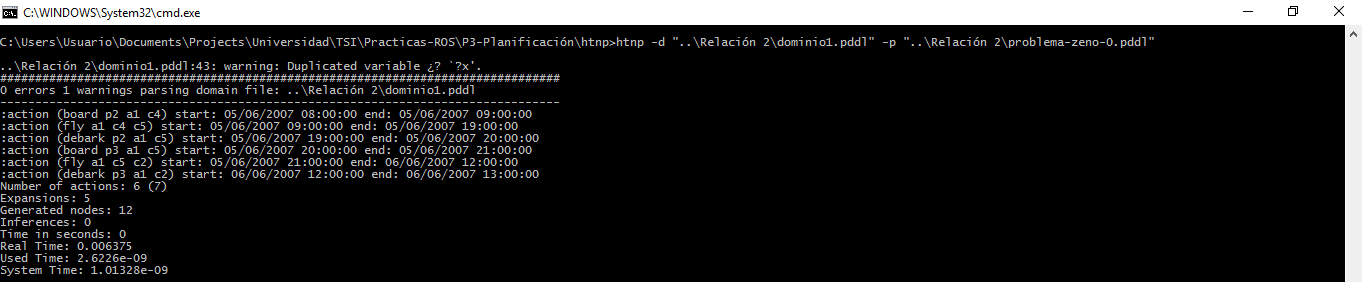
\includegraphics[width=15cm]{Ej1-problema0.png}
			\caption{Solución del problema 0.}
			\label{Prob-0}
		\end{figure}
		
	
	\subsection{Problema 1}
		El problema 1 consiste en transportar 3 personas inicialmente en distintas ciudades a una misma ciudad,
		sin restricciones de fuel.
		
		Inicialmente, podemos ver que el dominio aportado como ejemplo considera algunos casos para la tarea
		\textit{transport-person}, en concreto, registra los casos de que la persona ya se halle en la ciudad
		destino y el de que no esté en la ciudad destino pero sí en la del avión. Por tanto, sólo tenemos
		que implementar el caso de que no esté ni en la ciudad destino ni en la del avión, cuya solución sería
		mover el avión a dicha ciudad y luego actuar como en el caso anterior como podemos ver en el fichero
		\textit{dominio1.pddl}.
		
		Ahora, podemos comprobar que obtenemos un resultado para este problema:
		\begin{figure}[H]
			\centering
			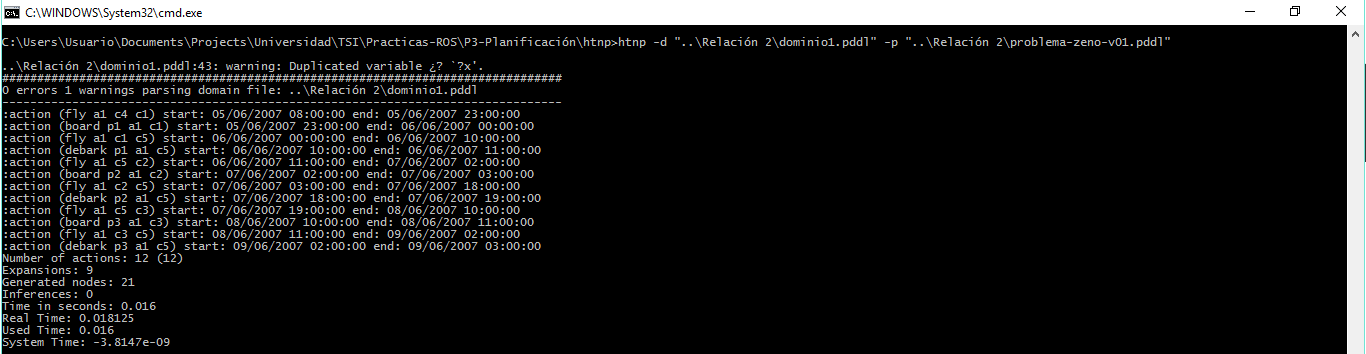
\includegraphics[width=15cm]{Ej1-problema1.png}
			\caption{Solución del problema 1.}
			\label{Prob-1}
		\end{figure}
		
	\subsection{Problema 2}
		El problema 2 consiste en consiste en asumir ahora que hay restricciones de fuel.
		
		La solución de estas circunstancias pasan por modificar la tarea \textit{mover-avion} en la que ya tenemos
		implementado el método que supone suficiente fuel y realizar la comprobación de que haya fuel antes de
		realizar el vuelo, en caso de que no lo hubiese, sería necesario repostar previamente y después, volar.
		
		Como podemos ver, estas simples acciones nos permiten resolver el segundo problema planteado:
		\begin{figure}[H]
			\centering
			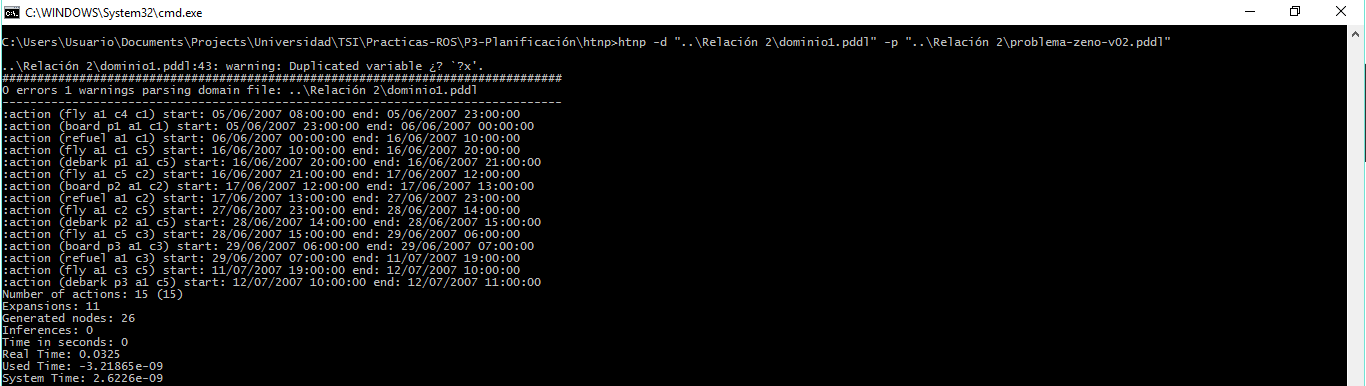
\includegraphics[width=15cm]{Ej1-problema2.png}
			\caption{Solución del problema 2.}
			\label{Prob-2}
		\end{figure}
		
	\subsection{Problema 3}
		El problema 3 consiste en considerar acciones de vuelo lento y rápido para tratar de transportar las
		personas lo más rápido posible sin exceder el límite de fuel.
		
		En esta ocasión, tenemos que plantear la bifurcación entre optar por volar a baja velocidad para
		conservar el máximo combustible posible, ya sea por falta de capacidad en el depósito o por evitar
		exceder el límite de fuel total impuesto.
		
		Simplemente, debemos añadir los predicados de \textit{hay-fuel-fast} en contraposición con
		\textit{hay-fuel-slow} que nos permite conocer si tenemos suficiente combustible en el depósito
		para realizar un vuelo rápido o lento, respectivamente. Junto con \textit{suficiente-fuel-fast} y
		\textit{suficiente-fuel-slow} para controlar no excedernos en el límite total de fuel consumido tras
		el viaje que estamos planeando hacer.
		
		Una vez definidos estos predicados derivados a partir de operaciones simples de suma, producto y
		comparación como podemos ver en el dominio, jugaremos con ellos para elegir entre los métodos de
		\textit{vuela-rapido}, \textit{vuela-lento} o incluso saber si es necesario repostar antes de
		\textit{vuela-rapido}.
		
		Finalmente, tras la implementación de estos métodos, podemos concluir que hemos resuelto los 3
		problemas que tenía el problema inicial como podemos verificar:
		\begin{figure}[H]
			\centering
			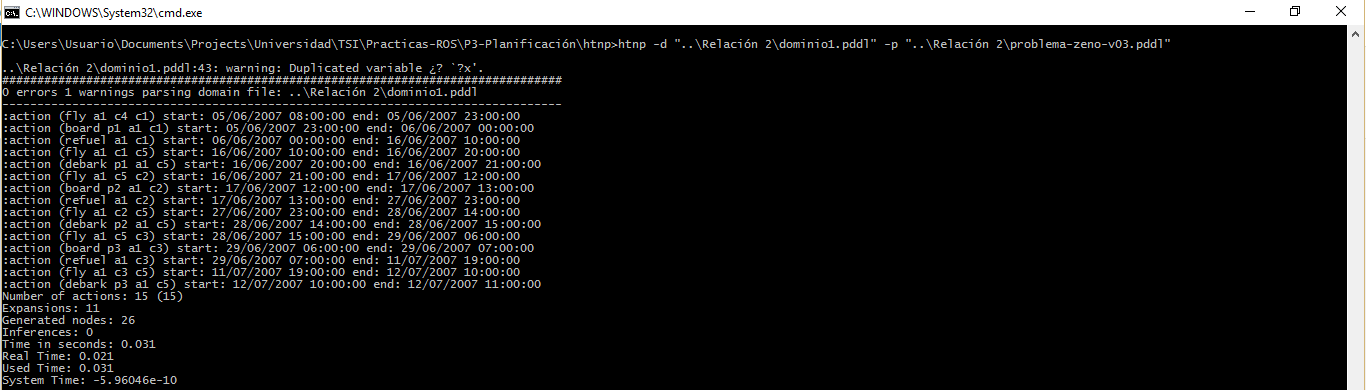
\includegraphics[width=15cm]{Ej1-problema3.png}
			\caption{Solución del problema 3.}
			\label{Prob-3}
		\end{figure}

\section{Dominio 2}
	\subsection{Implementar \textit{(distancia ?x ?y ?d)} como predicado derivado}
	\subsection{Modificar \textit{board} y \textit{debark} para permitir embarcar varios pasajeros}
	\subsection{Permitir embarcar varios pasajeros}
	\subsection{Duración limitada del viaje}


\end{document}
